\documentclass[conference]{IEEEtran}
\IEEEoverridecommandlockouts
% The preceding line is only needed to identify funding in the first footnote. If that is unneeded, please comment it out.
\usepackage{cite}
\usepackage{amsmath,amssymb,amsfonts}
\usepackage{algorithmic}
\usepackage{graphicx}
\usepackage{textcomp}
\usepackage{xcolor}
\def\BibTeX{{\rm B\kern-.05em{\sc i\kern-.025em b}\kern-.08em
    T\kern-.1667em\lower.7ex\hbox{E}\kern-.125emX}}
\begin{document}

\title{Hardware-aware Neural Architecture Search\\}

\author{\IEEEauthorblockN{Annika {\"O}sterdiekhoff}
\IEEEauthorblockA{\textit{Embedded Systems} \\
\textit{University Duisburg-Essen}\\
Duisburg, Germany \\
annika.oesterdiekhoff@stud.uni-due.de}
}

\maketitle

\begin{abstract}
Our goal is to give a brief overview about hardware-aware neural architecture search. 
\end{abstract}

\begin{IEEEkeywords}

\end{IEEEkeywords}

\section{Introduction}
Deep learning models are gaining more and more interest in ... (examples + citiation). These models consist of various layers and parameters. It is difficult for the developer to design the number and type of nodes and the connection between them because of the multiple differences in data types, tasks and hardware platforms. Therefore, most of the deep learning models are created by hand with multiple experiments or are a variation of already known models which work well. This process of creating and designing a model is very time-consuming, therefore techniques are created in the last years to automate the designing process of a deep learning model. It is called Neural Architecture Search (NAS). The focus of the survey is a subgroup of NAS, the hardware or platform-aware NAS (HW-NAS). The goal of HW-NAS is to use NAS for designing a deep learning model but with respect to optimize the deep learning model for a hardware device.  

\section{Neural Architecture Search Definition}
A neural architecture process firstly includes a search space which consists of possible operators and its connections which create a architecture. The search strategy explores this search space. Then the evaluation methodology is used to evaluate the accuracy of each model. The evaluation methodology trains the architecture and the models with a high accuracy help to redefine the search space. This training and in general the  number of architecture in forms of layers and parameters cause time consumption and large memory footprints. This leads to a lack of using NAS in real-time. 

\section{Model Optimizations}
For solving the drawbacks mentioned above  to get large deep learning models and long training processes, there are some techniques to optimize it.

Firstly you can compress a model. Compressing a model can be done for example by compact the model which changes the standard operations to more flexible and simpler operations. In addition, one can decompose the tensor which means we shrink the tensors which reduces the size of the deep learning model. What we will mainly focus on for compressing a model is quantization. Quantizations means that we convert floating point weights and activation's into smaller integers, ideally binaries. Another option for compressing a model is pruning where the least important weights or operations are pruned to reduce the model size. The importance of a weight or operation can be the weight itself or has to be learned. 

In addition one can apply hardware-aware NAS which uses model compression's and takes the hardware usability into account by design the model. A relatively new technique for optimizing a deep learning model is code transformation which optimizes the operators of an model.

\section{Hardware-Aware NAS Problem Formulation}
In the following we discuss the problem formulation of hardware-aware neural architecture search. In general, neural architecture search is an optimization problem which search for an architecture which maximizes a performance metrics. The performance metric is mostly the accuracy. The formulation is shown in ``\eqref{eqn:single-obj}''. 
 
\begin{equation}
\label{eqn:single-obj}
\max_{\alpha\epsilon A}\,f(\alpha, \delta)
\end{equation}

So, $A$ is the search space which includes the set of architectures and $\alpha$ is one architecture from this set. $\delta$ is the used data set and $f$ is the performance measure, i.e. the accuracy.  The formulation says that we try to find the architecture $\alpha$ of the search space $A$ which maximizes the accuracy $f$ for the used data set. 
 
By doing hardware-aware neural architecture search one has not only the accuracy metric which should be maximized but also hardware objectives like for example latency. There exist different problem formulation for hardware-aware neural architecture search, the single and multi-objective optimization.

\subsection{Single-Objective Optimization}

Single-objective optimization means that only one objective is maximized like explained above for example the accuracy. For solving the problem of also having hardware objectives one tries to transform the multi-objective optimization into a single-objective optimization. For doing this there exist two methods. Two-Stage optimization means that we use the problem formulation of original neural architecture search which maximizes the accuracy and optimize in the second stage the architecture for a specific target. This method often does not work well because the best founded architecture in the first stage is maybe not the best for the specific target hardware. The alternative to this method is constrained optimization. Here we again try to find the architecture with the highest accuracy but we define some thresholds for hardware constrains like latency or energy consumption which are not allowed to be exceeded by the founded architecture. 

\subsection{Multi-Objective Optimization}

The difference to the single-objective optimization which is used in original NAS is multi-objective optimization. The formulation is shown here: ``\eqref{eqn:multi-obj}''.
 
\begin{equation}
\label{eqn:multi-obj}
\max_{\alpha\epsilon A}\,f_{1}(\alpha, \delta),f_{2}(\alpha, \delta),\ldots ,f_{n}(\alpha, \delta)
\end{equation}     

So we now do not only have the accuracy which we have to optimize but various objectives, e.g. latency and energy consumption. These objectives can be conflicting each other for example try to have a minimal search space and gaining the best accuracy. When this occurs we can only try to find the Pareto-optimal solution. There exist two approaches for this. Firstly the scalarization method which includes the performance measurements $f$'s into one aggregation function like a weighted sum or weighted product. This transforms the multi-objective optimization into a single-objective optimization. Unfortunately by having fixed weights in the aggregation function, it could be that not all Pareto solutions are found. For solving this issue one can run multiple runs which on the other hand then again leads to more needed computing power etc. Another method to find the Pareto-optimal solution is defining heuristics. By doing this one does not form the multi-objective optimization problem into a single-objective one and therefore get a set of architectures as solutions along the Pareto front. 

explain pareto 

\section{Goals?}
There are three categories of goals of hardware-aware neural architecture search. Firstly, the category single target, fixed configurations where most hardware-aware NAS belongs to. Single target means that the neural architecture search tries to find the best architecture for one single target, for example for FPGAs. We divide this category further in hardware-aware search strategy and hardware-aware search space. The hardware-aware search strategy focuses on solving the neural architecture search as a multi-objective problem which means that the accuracy is taken into account as always but also some hardware measurements for example latency. The opposite to this is the hardware-aware search space where the neural architecture search works with only a pool of architectures. The bad working architectures on the target hardware are eliminated. It helps to have a prior knowledge for the target platform for creating the set of architectures. The neural architecture search considers then only the accuracy for this set of architectures and no hardware measurements.

The second category of goals of hardware-aware neural architecture search is single target, multiple configurations. This category focuses on searching the best architecture in terms of latency in combination to accuracy. 

configurations? what do they mean?

In addition, it exists the category multiple targets. This means one does not focus on one specific hardware like FPGAs but search for the best architecture for multiple hardware platforms. This approach is the most desirable one because it allows one to port the best architecture to different hardware platforms. But it is also the most challenging one because architectures perform differently on different hardware. 

\section{Search Spaces}

There exist two search spaces for the search strategies for hardware-aware neural architecture search. 

\subsection{Architecture Search Space}

The first one is the Architecture Search Space. It defines a set of architectures which means a set of possible operators and their connections. For designing an architecture search space one can use a fixed architecture and only search for the best hyper-parameters. Unfortunately this needs some knowledge of the human which designs the architecture, but it reduces the size of the search space. On the other hand one can do a search without a fixed architecture and search for fitting operators and their connections. This does not need knowledge of the human how the architecture structure should look like but of course it produces a bigger search space size and with this also a longer search time. By searching for the best architecture without a fixed architecture one distinguishes between three types. Firstly one can have a layer-wise search space where the architecture is searched out of a set of operators. Another option is to use a cell-based search space. A cell is defined as a graph that includes feature transformations. A cell-based search space creates a architecture by repeating these cells. This mostly leads to a high accuracy but it limits the flexibility in hardware specialization. In addition, there exists the hierarchical search space. The architecture is build by constructing blocks out of a defined number of cells. This solves the missing flexibility of the cell-based search space (WHY?). 

\subsection{Hardware Search Space}

The second possible search space is the Hardware Search Space. This means before evaluating the architecture one already does some hardware optimizations. It is not possible to do add all hardware specifications in the search space for optimizing because it would explode the search space and in combination the search space time. There exist three types of hardware search space. The search space can be parameter-based which means that the search space is a set of optimizing parameters. On the other hand a search space can be template-based. So the search space consists of a set of pre-configured templates instead of optimizing parameters. In general, one uses existing successful designs as templates.

third one???

\section{Search Strategies}

The search strategy consists of three elements: an accuracy evaluation method, a hardware cost evaluation method and a search algorithm. 

\subsection{Accuracy Evaluation Method}
The accuracy is evaluated by training the architectures of the search space and comparing the accuracy. Because it would be very time and computational consuming there exits some methods for estimate the accuracy without a training. First, weight sharing....

Second method for speeding up the determination of the accuracy is early stopping. This means one train a deep learning model only a few epochs and use the accuracy as an approximation for a complete training. In addition, one can include hot start. This means that the searching and training of an architecture is not started with a random model but with an efficient model. Examples for this efficient start models are ProxylessNAS and MNASNet models. Furthermore, proxy data set can be used to only train the deep learning model with fewer data elements and increase it in the last steps. In the end there also exits already some accuracy prediction models which use the architecture and data set for predicting the accuracy beforehand. Example prediction models are Peephole, PNAS or NeuNetS. 

\subsection{Hardware Cost Evaluation Method}
Hardware cost evaluation methods are methods for measuring hardware metrics in real-time or as an estimation. Possible hardware measurements are: 

\begin{itemize}
\item FLOPs and Model Size: FLOPs are floating point operations. This means the number of floating point operations and the number of parameters as the model size are used as hardware cost measurement. Unfortunately, the number of FLOPs do not completely correlate with the execution time. This means, FLOPs are not a good indicator to search for efficient architectures, but a small model size leads to fewer memory consumption and automatically searches for compressed models. 
\item Latency: A low latency is important for using NAS in real world applications for ensuring a fast action. 
\item Energy Consumption: The energy consumption measurement can be used as metric for hardware cost evaluation. Possibilities are to use the peak of an energy consumption or the average consumption.
\item Area: Area means that it is desired to take into account by evaluating the hardware cost to gain the smallest possible chip. The area also correlates with the power consumption as well.
\item Memory footprint: As said above the number of parameters from a model is a good indicator for measuring the memory footprint. Another better option is to measure the memory consumption while running.     
\end{itemize}

\subsubsection{Real World Measurements versus Estimation models}

Of course real world measurements are very good for evaluating the hardware cost because we are getting a very precise accuracy in comparison to the actual using. But real world measurements have some drawbacks. Mostly, it is very costly. One has to have all used hardware platforms available. In addition, the searching for the best architecture runs longer by getting more precise accuracy. Therefore, there exits estimation models like prediction models, lookup tables or a computation of an analytical estimation. The problem of creating estimation models is that the developer needs hardware experiences and knowledge for making an estimation about the hardware cost. In general, prediction models speed up the search time the most. After this follow the lookup tables and then the analytical estimation. 

\subsection{Search Algorithm}
The search algorithm samples the architectures from the search space and updates the search space for getting architectures with a higher accuracy.
In the following, we explain the two most used search algorithms in neural architecture search, namely reinforcement learning and evolutionary algorithms. By using reinforcement learning an agent chooses between actions in an environment and gets an reward after the action. Its goal is to maximizes the reward. In contrast to this are the evolutionary algorithms. They have three main characteristics: population-based, fitness-oriented and generations. Population-based means that the algorithm has a set of candidate solutions which are known as population. Fitness-oriented means that each solution has a quality which is express with its fitness score. In addition, the evolutionary algorithms create mutations and crossover operations to gain new populations.

Other possible search algorithms are for example gradient-based methods. Instead of separating the search and the evaluation one create a super-network which can simulate any child model. So parts of the model can share their weights which reduces the search time. By training the super-network one gets the weights and parameters for all child architectures. Another option is random search and Bayesian optimization which is the easiest by just randomly search an architecture but it consumes a lot of time in searching. 

Non-differentiable hardware constrains???

\section{Target Hardware Platforms}
There exits three different categories of target hardware platforms. Firstly the server processors which can be CPUs, GPUs, FPGAs and ASICs. Its goal is to maximize the accuracy. There is a increasing interest in adapting the neural architecture search for a specific hardware, but mostly up to now researcher do not take into account the constraints of each hardware platform. The second category are mobile devices which are widely used but do not have much memory and computational power. Therefore, more and more research is focused on gaining high accuracy by using constrained hardware. The last category are tiny devices which are devices that run deep learning model with very low power. 

\section{???}

As described above there exits multiple approaches to reduce the memory footprint and execution time. There are two techniques for gaining this goal, handcrafting new more efficient operators and using deep learning optimizations. By focusing on the deep learning optimization used by neural architecture search, there exits automatic mixed-precision quantization as well as automatic pruning. Automatic mixed-precision quantization uses different bitwidths like binary or 8-bit precision for different layers for activation function and weights. By reducing the memory footprint, this approach does not reduce the search space and the computations. In addition specific MAC architectures with scalable-precision are needed which restricts the power efficiency. On the other hand automatic pruning is used in neural architecture search by pruning the least important neurons. 

\section{NAS Frameworks}

There are multiple frameworks for doing neural architecture search, for example Auto-Keras, Google AutoML, IBM NeuNets, TPOT, Microsoft Archai, deci.ai AutoNAC, Darwin and Microsoft NNI. All these frameworks have their advantages and disadvantages and focus on different use-cases. We focus on the Microsoft Neural Network Intelligence (NNI) framework. (WHY?) Microsoft NNI can be used to better compare, reproduce and experiment with various NAS algorithms. It helps the researcher to design their neural network architecture for example by helping by the definition of a super network. It concentrates on the efficiency of the automation by doing neural architecture search. In addition, researcher can use existing NAS algorithms and can easily modify them. Except for AutoNAC, all existing frameworks are not hardware-aware, but Google AutoML and Microsoft NNI support compression methods for specializing the target platform. 

\section{Challenges and Limitations}

In the following we list various challenges and limitations of hardware-aware neural architecture search. 

\subsection{Benchmarking and Reproducibility}

For providing comparison, it should be possible to reproduce neural architecture search. But this is difficult because of the huge possibilities of search spaces, training methods, computational resources and especially for hardware-aware NAS possibilities of hardware devices. For solving this problem there are set some benchmarks. Firstly, researchers should directly query a tabular data set instead of generating a search space for reducing the needed costs. In addition, it should be used various search strategies on the same search space for a relatable comparing between the strategies. Furthermore, data sets which are used by accuracy predictor models and hardware cost models should be provided. Also, make NAS easier for developers without hardware knowledge by proposing data sets with hardware-related metrics.

\subsection{Transferability of AI Models}

Transferability means to train a model on one data set and fine-tune it after that on the target data set. Reasons for doing this are that one can use a simpler and smaller train data set or if the target data set has not enough data points for training. 

Most researchers use cell-based search space in neural architecture search for transfer their model. For transferring, you modify the network by adding more cells and adjust the input sizes of the cells. Some recent works start to transfer hierarchical search space by varying the cells and operators of each cell. Another option is to discard the fine-tuning and directly find transferable weights. For this one create a task-specific super-network from an overall super-network and search then for architectures within this task. Therefore, no extra training is needed. 

In general, transfer a model in NAS is very difficult. A starting point is to create a macro-architecture for a specific task and modify the search space for this task. By considering the hardware, one has to transfer to different hardware platforms which is on top not easy. 
 
\subsection{Transferability of the hardware-aware NAS across multiple Platforms}

One interesting topic in hardware-aware neural architecture search is to design an architecture and transfer it to multiple different platforms. The problem hereby is the variety and different complexities of the hardware platforms. For solving this issue there exits two approaches.

\subsubsection{Transfer the entire NAS Process}

The idea is to transfer a NAS to a different hardware platform by changing the measurement values. For this the whole NAS process is run again on the different hardware. This rerun of the NAS process leads to high computational consumption's. In addition, it can be a huge effort to collect the hardware constraints. The hardware measurements can be done with real-world measurements, analytical estimation, lookup tables and prediction models like explained above. But real-world measurements need the target hardware platform already during search time and are very slow. Analytical estimation needs experiences from the developer in the specific target hardware whereas lookup tables and prediction models have to run the complete set of operators again. Therefore, all in all it is very difficult and not scalable to transfer a NAS process to a new hardware by changing the measurement values. 

\subsubsection{Transfer the final Model}

The second approach is to transform a final model of a NAS process to fit to a different hardware. For fitting the final architecture to a smaller device, mostly compressing the model is used. But this specialization has some limits. Firstly, different operators are not equally efficient for two different platforms. This also makes hardware-aware NAS which tries to find the best architecture for multiple hardware platforms difficult. In addition, there are limits in the compression methods. Compressed models never lead to a higher accuracy as the original model. 

\section{Conclusion}

\clearpage

\section{Introduction}
This document is a model and instructions for \LaTeX.
Please observe the conference page limits. 

\section{Ease of Use}

\subsection{Maintaining the Integrity of the Specifications}

The IEEEtran class file is used to format your paper and style the text. All margins, 
column widths, line spaces, and text fonts are prescribed; please do not 
alter them. You may note peculiarities. For example, the head margin
measures proportionately more than is customary. This measurement 
and others are deliberate, using specifications that anticipate your paper 
as one part of the entire proceedings, and not as an independent document. 
Please do not revise any of the current designations.

\section{Prepare Your Paper Before Styling}
Before you begin to format your paper, first write and save the content as a 
separate text file. Complete all content and organizational editing before 
formatting. Please note sections \ref{AA}--\ref{SCM} below for more information on 
proofreading, spelling and grammar.

Keep your text and graphic files separate until after the text has been 
formatted and styled. Do not number text heads---{\LaTeX} will do that 
for you.

\subsection{Abbreviations and Acronyms}\label{AA}
Define abbreviations and acronyms the first time they are used in the text, 
even after they have been defined in the abstract. Abbreviations such as 
IEEE, SI, MKS, CGS, ac, dc, and rms do not have to be defined. Do not use 
abbreviations in the title or heads unless they are unavoidable.

\subsection{Units}
\begin{itemize}
\item Use either SI (MKS) or CGS as primary units. (SI units are encouraged.) English units may be used as secondary units (in parentheses). An exception would be the use of English units as identifiers in trade, such as ``3.5-inch disk drive''.
\item Avoid combining SI and CGS units, such as current in amperes and magnetic field in oersteds. This often leads to confusion because equations do not balance dimensionally. If you must use mixed units, clearly state the units for each quantity that you use in an equation.
\item Do not mix complete spellings and abbreviations of units: ``Wb/m\textsuperscript{2}'' or ``webers per square meter'', not ``webers/m\textsuperscript{2}''. Spell out units when they appear in text: ``. . . a few henries'', not ``. . . a few H''.
\item Use a zero before decimal points: ``0.25'', not ``.25''. Use ``cm\textsuperscript{3}'', not ``cc''.)
\end{itemize}

\subsection{Equations}
Number equations consecutively. To make your 
equations more compact, you may use the solidus (~/~), the exp function, or 
appropriate exponents. Italicize Roman symbols for quantities and variables, 
but not Greek symbols. Use a long dash rather than a hyphen for a minus 
sign. Punctuate equations with commas or periods when they are part of a 
sentence, as in:
\begin{equation}
a+b=\gamma\label{eq}
\end{equation}

Be sure that the 
symbols in your equation have been defined before or immediately following 
the equation. Use ``\eqref{eq}'', not ``Eq.~\eqref{eq}'' or ``equation \eqref{eq}'', except at 
the beginning of a sentence: ``Equation \eqref{eq} is . . .''

\subsection{\LaTeX-Specific Advice}

Please use ``soft'' (e.g., \verb|\eqref{Eq}|) cross references instead
of ``hard'' references (e.g., \verb|(1)|). That will make it possible
to combine sections, add equations, or change the order of figures or
citations without having to go through the file line by line.

Please don't use the \verb|{eqnarray}| equation environment. Use
\verb|{align}| or \verb|{IEEEeqnarray}| instead. The \verb|{eqnarray}|
environment leaves unsightly spaces around relation symbols.

Please note that the \verb|{subequations}| environment in {\LaTeX}
will increment the main equation counter even when there are no
equation numbers displayed. If you forget that, you might write an
article in which the equation numbers skip from (17) to (20), causing
the copy editors to wonder if you've discovered a new method of
counting.

{\BibTeX} does not work by magic. It doesn't get the bibliographic
data from thin air but from .bib files. If you use {\BibTeX} to produce a
bibliography you must send the .bib files. 

{\LaTeX} can't read your mind. If you assign the same label to a
subsubsection and a table, you might find that Table I has been cross
referenced as Table IV-B3. 

{\LaTeX} does not have precognitive abilities. If you put a
\verb|\label| command before the command that updates the counter it's
supposed to be using, the label will pick up the last counter to be
cross referenced instead. In particular, a \verb|\label| command
should not go before the caption of a figure or a table.

Do not use \verb|\nonumber| inside the \verb|{array}| environment. It
will not stop equation numbers inside \verb|{array}| (there won't be
any anyway) and it might stop a wanted equation number in the
surrounding equation.

\subsection{Some Common Mistakes}\label{SCM}
\begin{itemize}
\item The word ``data'' is plural, not singular.
\item The subscript for the permeability of vacuum $\mu_{0}$, and other common scientific constants, is zero with subscript formatting, not a lowercase letter ``o''.
\item In American English, commas, semicolons, periods, question and exclamation marks are located within quotation marks only when a complete thought or name is cited, such as a title or full quotation. When quotation marks are used, instead of a bold or italic typeface, to highlight a word or phrase, punctuation should appear outside of the quotation marks. A parenthetical phrase or statement at the end of a sentence is punctuated outside of the closing parenthesis (like this). (A parenthetical sentence is punctuated within the parentheses.)
\item A graph within a graph is an ``inset'', not an ``insert''. The word alternatively is preferred to the word ``alternately'' (unless you really mean something that alternates).
\item Do not use the word ``essentially'' to mean ``approximately'' or ``effectively''.
\item In your paper title, if the words ``that uses'' can accurately replace the word ``using'', capitalize the ``u''; if not, keep using lower-cased.
\item Be aware of the different meanings of the homophones ``affect'' and ``effect'', ``complement'' and ``compliment'', ``discreet'' and ``discrete'', ``principal'' and ``principle''.
\item Do not confuse ``imply'' and ``infer''.
\item The prefix ``non'' is not a word; it should be joined to the word it modifies, usually without a hyphen.
\item There is no period after the ``et'' in the Latin abbreviation ``et al.''.
\item The abbreviation ``i.e.'' means ``that is'', and the abbreviation ``e.g.'' means ``for example''.
\end{itemize}
An excellent style manual for science writers is \cite{b7}.

\subsection{Authors and Affiliations}
\textbf{The class file is designed for, but not limited to, six authors.} A 
minimum of one author is required for all conference articles. Author names 
should be listed starting from left to right and then moving down to the 
next line. This is the author sequence that will be used in future citations 
and by indexing services. Names should not be listed in columns nor group by 
affiliation. Please keep your affiliations as succinct as possible (for 
example, do not differentiate among departments of the same organization).

\subsection{Identify the Headings}
Headings, or heads, are organizational devices that guide the reader through 
your paper. There are two types: component heads and text heads.

Component heads identify the different components of your paper and are not 
topically subordinate to each other. Examples include Acknowledgments and 
References and, for these, the correct style to use is ``Heading 5''. Use 
``figure caption'' for your Figure captions, and ``table head'' for your 
table title. Run-in heads, such as ``Abstract'', will require you to apply a 
style (in this case, italic) in addition to the style provided by the drop 
down menu to differentiate the head from the text.

Text heads organize the topics on a relational, hierarchical basis. For 
example, the paper title is the primary text head because all subsequent 
material relates and elaborates on this one topic. If there are two or more 
sub-topics, the next level head (uppercase Roman numerals) should be used 
and, conversely, if there are not at least two sub-topics, then no subheads 
should be introduced.

\subsection{Figures and Tables}
\paragraph{Positioning Figures and Tables} Place figures and tables at the top and 
bottom of columns. Avoid placing them in the middle of columns. Large 
figures and tables may span across both columns. Figure captions should be 
below the figures; table heads should appear above the tables. Insert 
figures and tables after they are cited in the text. Use the abbreviation 
``Fig.~\ref{fig}'', even at the beginning of a sentence.

\begin{table}[htbp]
\caption{Table Type Styles}
\begin{center}
\begin{tabular}{|c|c|c|c|}
\hline
\textbf{Table}&\multicolumn{3}{|c|}{\textbf{Table Column Head}} \\
\cline{2-4} 
\textbf{Head} & \textbf{\textit{Table column subhead}}& \textbf{\textit{Subhead}}& \textbf{\textit{Subhead}} \\
\hline
copy& More table copy$^{\mathrm{a}}$& &  \\
\hline
\multicolumn{4}{l}{$^{\mathrm{a}}$Sample of a Table footnote.}
\end{tabular}
\label{tab1}
\end{center}
\end{table}

\begin{figure}[htbp]
\centerline{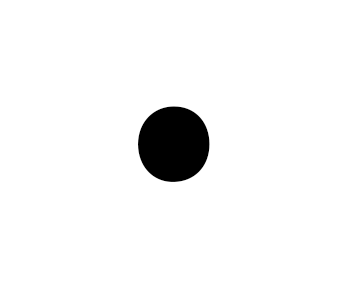
\includegraphics{fig1.png}}
\caption{Example of a figure caption.}
\label{fig}
\end{figure}

Figure Labels: Use 8 point Times New Roman for Figure labels. Use words 
rather than symbols or abbreviations when writing Figure axis labels to 
avoid confusing the reader. As an example, write the quantity 
``Magnetization'', or ``Magnetization, M'', not just ``M''. If including 
units in the label, present them within parentheses. Do not label axes only 
with units. In the example, write ``Magnetization (A/m)'' or ``Magnetization 
\{A[m(1)]\}'', not just ``A/m''. Do not label axes with a ratio of 
quantities and units. For example, write ``Temperature (K)'', not 
``Temperature/K''.

\section*{Acknowledgment}

The preferred spelling of the word ``acknowledgment'' in America is without 
an ``e'' after the ``g''. Avoid the stilted expression ``one of us (R. B. 
G.) thanks $\ldots$''. Instead, try ``R. B. G. thanks$\ldots$''. Put sponsor 
acknowledgments in the unnumbered footnote on the first page.

\section*{References}

Please number citations consecutively within brackets \cite{b1}. The 
sentence punctuation follows the bracket \cite{b2}. Refer simply to the reference 
number, as in \cite{b3}---do not use ``Ref. \cite{b3}'' or ``reference \cite{b3}'' except at 
the beginning of a sentence: ``Reference \cite{b3} was the first $\ldots$''

Number footnotes separately in superscripts. Place the actual footnote at 
the bottom of the column in which it was cited. Do not put footnotes in the 
abstract or reference list. Use letters for table footnotes.

Unless there are six authors or more give all authors' names; do not use 
``et al.''. Papers that have not been published, even if they have been 
submitted for publication, should be cited as ``unpublished'' \cite{b4}. Papers 
that have been accepted for publication should be cited as ``in press'' \cite{b5}. 
Capitalize only the first word in a paper title, except for proper nouns and 
element symbols.

For papers published in translation journals, please give the English 
citation first, followed by the original foreign-language citation \cite{b6}.

\begin{thebibliography}{00}
\bibitem{b1} G. Eason, B. Noble, and I. N. Sneddon, ``On certain integrals of Lipschitz-Hankel type involving products of Bessel functions,'' Phil. Trans. Roy. Soc. London, vol. A247, pp. 529--551, April 1955.
\bibitem{b2} J. Clerk Maxwell, A Treatise on Electricity and Magnetism, 3rd ed., vol. 2. Oxford: Clarendon, 1892, pp.68--73.
\bibitem{b3} I. S. Jacobs and C. P. Bean, ``Fine particles, thin films and exchange anisotropy,'' in Magnetism, vol. III, G. T. Rado and H. Suhl, Eds. New York: Academic, 1963, pp. 271--350.
\bibitem{b4} K. Elissa, ``Title of paper if known,'' unpublished.
\bibitem{b5} R. Nicole, ``Title of paper with only first word capitalized,'' J. Name Stand. Abbrev., in press.
\bibitem{b6} Y. Yorozu, M. Hirano, K. Oka, and Y. Tagawa, ``Electron spectroscopy studies on magneto-optical media and plastic substrate interface,'' IEEE Transl. J. Magn. Japan, vol. 2, pp. 740--741, August 1987 [Digests 9th Annual Conf. Magnetics Japan, p. 301, 1982].
\bibitem{b7} M. Young, The Technical Writer's Handbook. Mill Valley, CA: University Science, 1989.
\end{thebibliography}
\vspace{12pt}
\color{red}
IEEE conference templates contain guidance text for composing and formatting conference papers. Please ensure that all template text is removed from your conference paper prior to submission to the conference. Failure to remove the template text from your paper may result in your paper not being published.

\end{document}
